\documentclass[a4paper]{article}

\usepackage{polski}
\usepackage[utf8]{inputenc}
\usepackage[pdftex]{graphicx}
\usepackage{fancyhdr}
\usepackage{float}

\newcommand{\prog}{\texttt}

\linespread{1.15}
\pagestyle{fancy}
\fancyhf{}
\chead{Sprawozdanie końcowe}
\cfoot{Strona \thepage \ z \pageref{end}}

\title{Sprawozdanie końcowe \\ Projekt \textit{Aplikacja OnePass} w języku Python}
\author{Jakub Czajka (299239)}

\begin{document}
\maketitle
\tableofcontents
\thispagestyle{empty}
\newpage

\section{Wprowadzenie teoretyczne}
Moim zadaniem było stworzenie aplikacji realizującą usługę menadżera haseł. Mój program nazwałem \textit{OnePass}. Program inspirowana jest aplikacjami:
\begin{itemize}
    \item LastPass
    \item 1Password
\end{itemize}
Po uruchomieniu aplikacja pokazuje się menu główne. W tym menu możemy wybrać opcje zalogowania się, rejestracji lub przejść do generatora haseł.\\ \\
Jeżeli mamy już konto założone mamy możliwość zalogowania się do aplikacji i rozpoczęcia w niej pracy. Kiedy pierwszy raz uruchamiamy aplikację musimy się zarejestrować. Aplikacja wymusza na nas utworzenie trudnego do złamania hasła. Po rejestracji przenoszeni jesteśmy do głównego ekranu aplikacji.\\ \\
W tym miejscu zaczyna się główna funkcjonalność programu. Mamy możliwość przechowywania haseł do różnych serwisów, tworzenie szyfrowanych notatek oraz możemy szyfrować pliki przez nas podane. Dodatkowo aplikacja umożliwia łatwy sposób na skopiowanie hasła, którego akurat potrzebujemy. Wszystko zależy od nas co będziemy przechowywać w aplikacji.\\ \\
Kiedy skończymy pracę wystarczy kliknąć przycisk \textit{Wyloguj} by wszystkie nasze informacje, które zapisaliśmy w aplikacji, zostały zaszyfrowane. Dostęp do tych plików mamy wyłącznie z aplikacji.
\\
\begin{figure}[H]
    \centering
    
\includegraphics[width = 0.5\textwidth]{img/ikona.png}
    \caption{Ikona programu}
    \label{fig:ikona}
\end{figure}

\section{Jakie założenia wstępne udało się spełnić?}
Udało mi się zaimplementować w programie prawie wszystkie przewidywane funkcjonalności. Lista poniżej przedstawia jakie one są:
\begin{enumerate}
    \item Utworzenie nowego użytkownika.
    \item Wczytywanie plików.
    \item Możliwość szyfrowania podanych przez użytkownika plików.
    \item Możliwość deszyfrowania podanych przez użytkownika plików.
    \item Zapisywanie haseł użytkowników w postaci haszy.
    \item Szyfrowanie plików.
    \item Deszyfrowanie plików.
    \item Możliwość edycji profilu.
    \item Zablokowanie zmiany hasła na hasło niebezpieczne.
    \item Możliwość generowania haseł.
    \item Możliwość wczytania jedynie plików przewidywanych przez program.
    \item Obsługa błędów powstałych na skutek wprowadzania niepoprawnych ciągów znaków w pola przy tworzeniu użytkownika i zmiany informacji o profilu.
    \item Możliwość wyświetlenia wszystkich okien.
    \item Zbudowanie rozbudowanego interfejsu graficznego.
    \item Możliwość usuwania notatek.
    \item Możliwość edycji notatek.
    \item Możliwość dodania nowych haseł do banku haseł.
    \item Możliwość edycji haseł w banku haseł.
\end{enumerate}

\section{Jakich zadań nie udało się zrealizować?}
Niestety nie wszystkie założenia i cele zostały przeze mnie w pełni zrealizowane. Jest to przede wszystkim:
\begin{enumerate}
    \item Zaimplementowanie mechanizmu blokady / odblokowywania konta w razie niepożądanej próby dostępu.
    \item Możliwości zaszyfrowania różnych rozszerzeń plików.
    \item Zachowanie systematyczności pisania testów programu.
    \item Uniknięcie zmian podczas kodowania w stosunku do specyfikacji implementacyjnej.
    \item Przetestowanie działania programu w systemie operacyjnym MacOS X i Linux.
    \item Napisanie integracji aplikacji z przeglądarkami.
    \item Możliwości usuwania haseł z banku haseł.
    \item Wyświetlania polskich znaków w notatkach.
    \item Możliwości pełnej edycji haseł z banku haseł.
    \item Dodania filtra w banku haseł.
    \item Zaimplementowanie systemu resetowania hasła.
\end{enumerate}
\newpage
\section{Przykładowe uruchomienia}
Poniższe ilustracje przedstawiają przykładowe ekrany działania programu:
\begin{figure}[H]
    \centering
    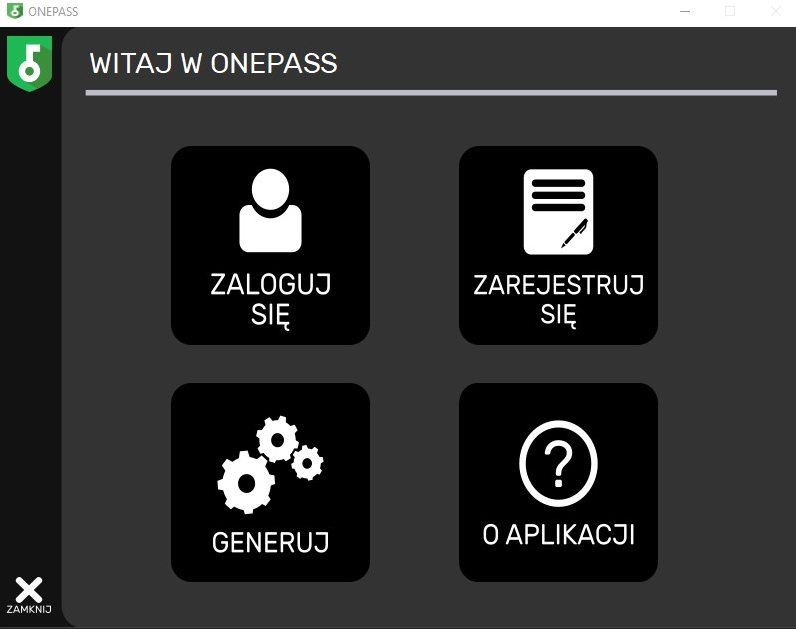
\includegraphics[width=1\textwidth]{img/ekran_glowny.png}
    \caption{Ekran główny przed zalogowaniem}
\end{figure}

\begin{figure}[H]
    \centering
    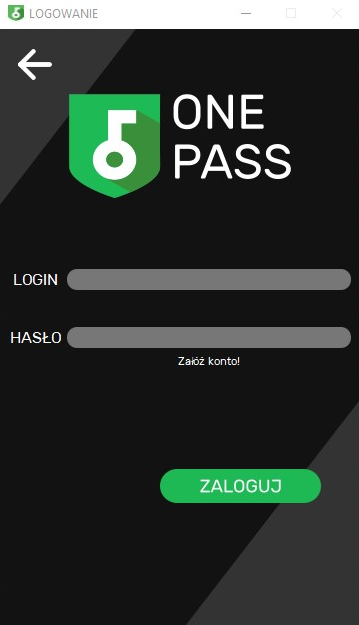
\includegraphics[height=1\textwidth]{img/ekran_zaloguj.png}
    \caption{Ekran logowania}
\end{figure}

\begin{figure}[H]
    \centering
    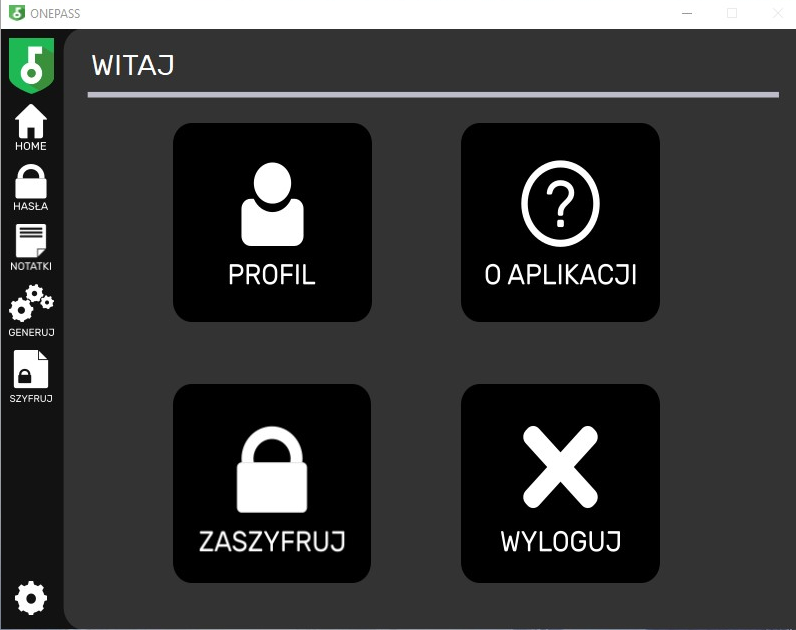
\includegraphics[width=1\textwidth]{img/ekran_glowny_po.jpg.png}
    \caption{Ekran główny po zalogowaniu}
\end{figure}

\begin{figure}[H]
    \centering
    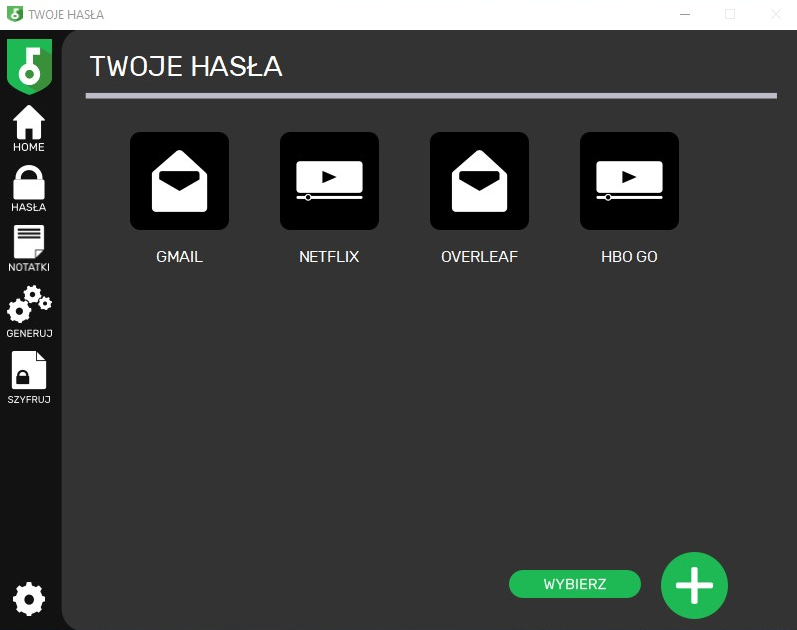
\includegraphics[width=1\textwidth]{img/ekran_hasla.png}
    \caption{Ekran haseł}
\end{figure}

\begin{figure}[H]
    \centering
    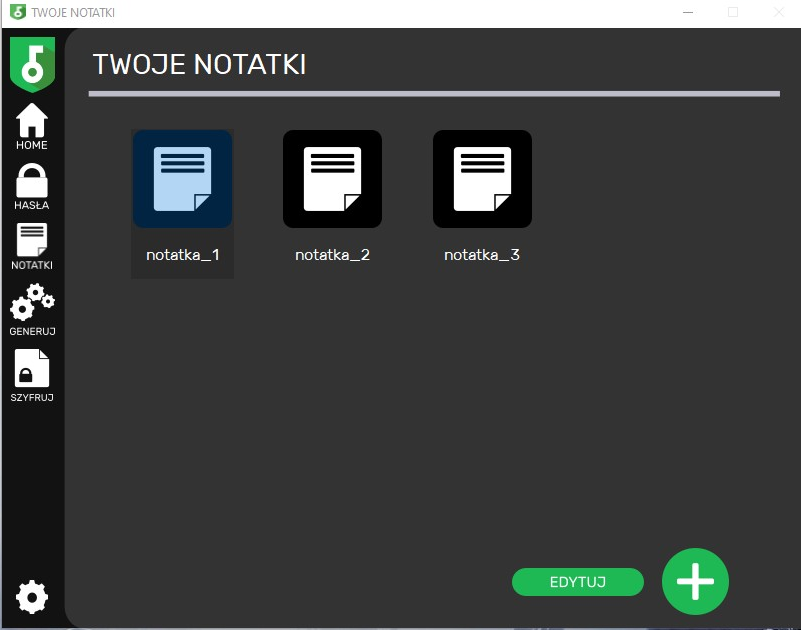
\includegraphics[width=1\textwidth]{img/ekran_notatek.png}
    \caption{Ekran notatek}
\end{figure}

\begin{figure}[H]
    \centering
    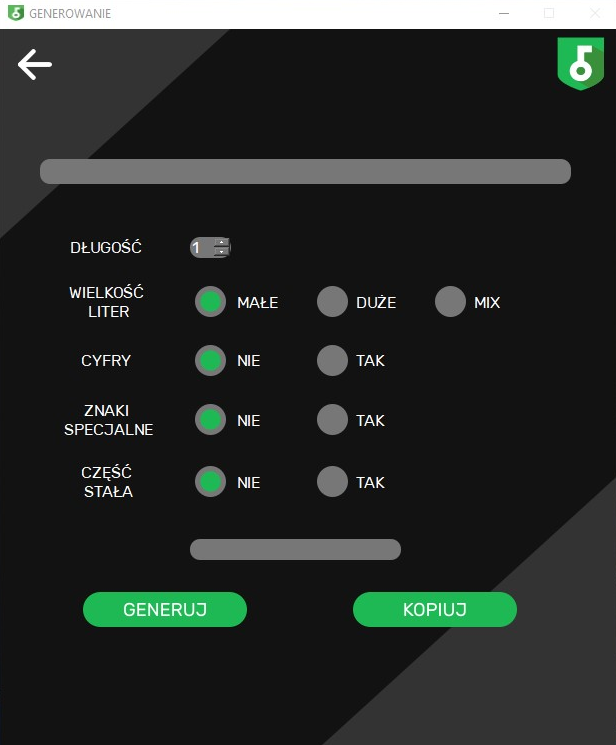
\includegraphics[height=1\textwidth]{img/ekran_generuj.png}
    \caption{Ekran generowania haseł}
\end{figure}

\begin{figure}[H]
    \centering
    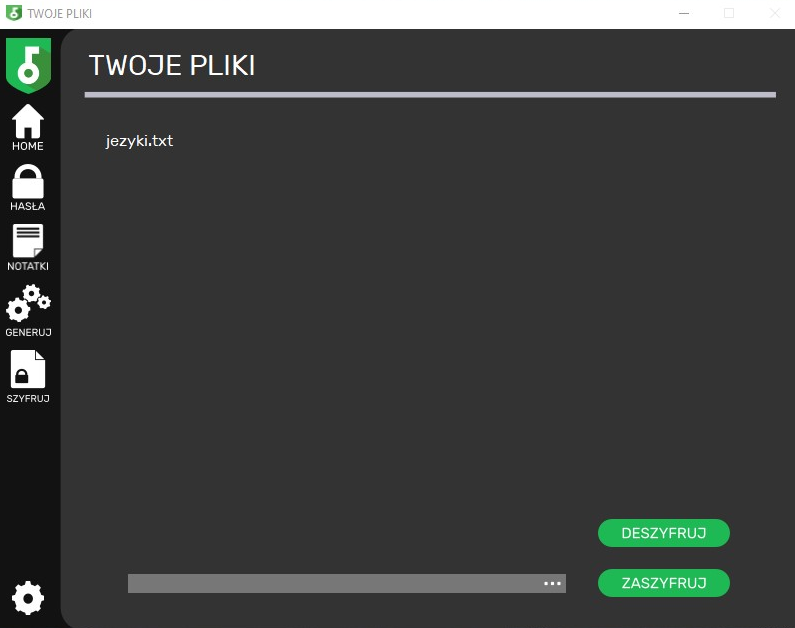
\includegraphics[width=1\textwidth]{img/ekran_szyfruj.png}
    \caption{Ekran szyfrowania plików}
\end{figure}

\section{Rozbieżności względem specyfikacji}
\subsection{Specyfikacja funkcjonalna}
Dodane zostało wczytywanie dwóch plików zawierających nazwy notatek oraz nazwy plików zaszyfrowanych. Ich zawartość wygląda następująco:\\ \\
\prog{NazwaNotatki1;NazwaNotatki2;...;NazwaNotatkiN}\\ \\
Struktura pliku z nazwami plików zaszyfrowanych ma postać:\\ \\
\prog{NazwaPliku1;NazwaPliku2;...NazwaPlikuN}


\subsection{Specyfikacja implementacyjna}
\begin{enumerate}
    \item Rozszerzenie klas o dodatkowe metody oraz pola, tak aby kod był napisany w sposób jak najbardziej optymalny i uniwersalny.
    \item Zmiana planowanych metod oraz pól w klasach spowodowana złym zaplanowaniem ich działania.
    \item Dodanie klas \prog{VWindow} i \prog{PController}, po których dziedziczą odpowiednio wszystkie klasy pakietu \textit{view} i \textit{controller}
    \item Rozdzielenie klasy \prog{VGenerateWin} i \prog{PGenerateWin} na dwie klasy odpowiednio wyświetlane przed oraz po zalogowaniu.
    \item Rozdzielenie klasy \prog{VAboutAppWin} i \prog{PAboutAppWin} na dwie klasy odpowiednio wyświetlane przed oraz po zalogowaniu.
    \item Drobne zmiany wyglądu GUI.
    \item Zmiany rozmieszczenia elementów GUI
    \item Zmiejsze liczby testów jednostkowych spowodowanych trudnością przeprowadzenia tych testów.
\end{enumerate}
\newpage

\section{Aktualna wersja diagramu klas}
Ze względu na rozmiar diagramu klas rozbiłem go na trzy diagramy dla poszczególnych pakietów:
\begin{figure}[H]
    \centering
    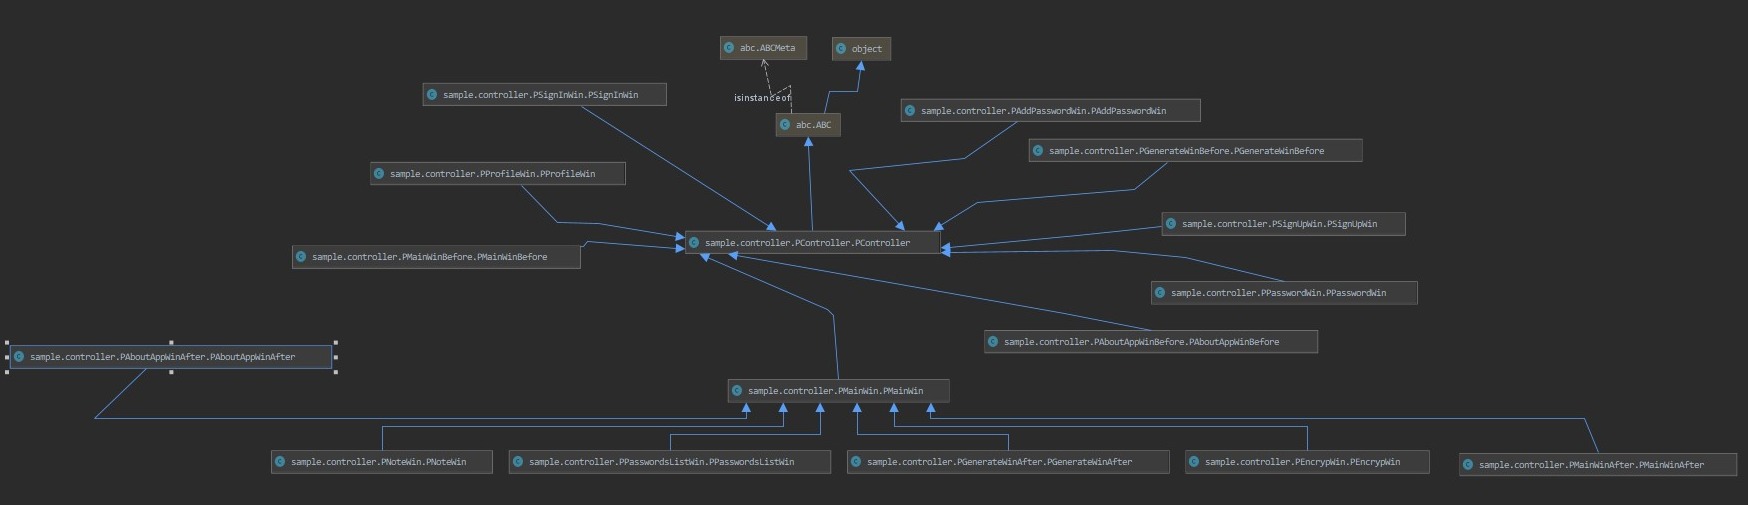
\includegraphics[width=1\textwidth, height=0.2\textheight]{img/diagram_con.png}
    \caption{Diagram klas pakietu \textit{Controller}}
\end{figure}

\begin{figure}[H]
    \centering
    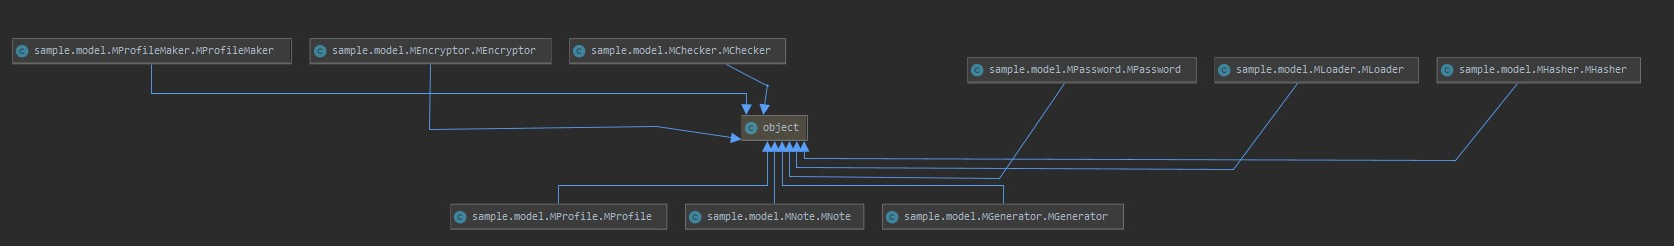
\includegraphics[width=1\textwidth]{img/diagram_mod.png}
    \caption{Diagram klas pakietu \textit{Model}}
\end{figure}

\begin{figure}[H]
    \centering
    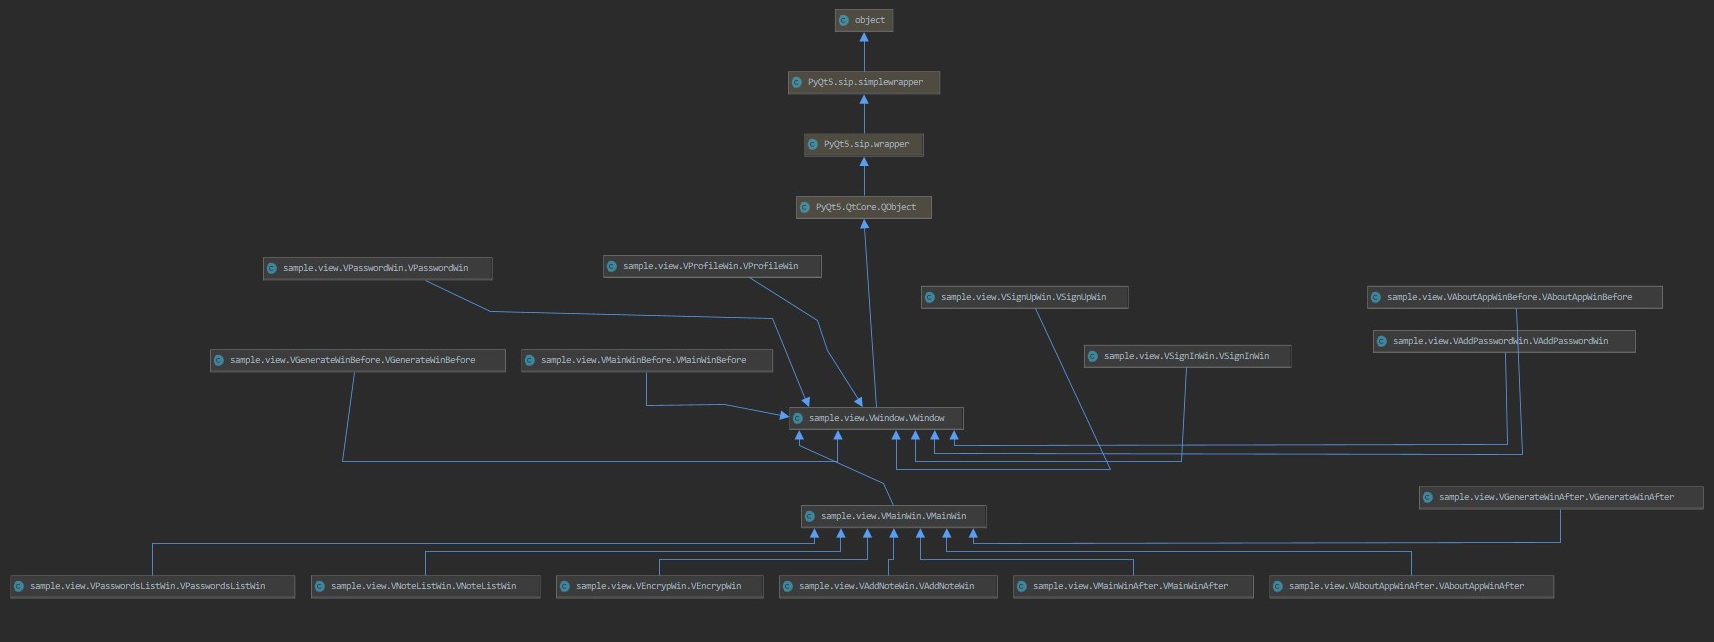
\includegraphics[width=1\textwidth, height=0.2\textheight]{img/diagram_view.png}
    \caption{Diagram klas pakietu \textit{View}}
\end{figure}

\section{Testy programu}
\paragraph{}
Funkcjonalność poszczególnych elementów programu sprawdzałem na bieżąco podczas implementacji.
Jeżeli dany komponent działał zgodnie z założeniami, dołączałem go do programu.
Dodatkowo dla klas pakietu \textit{model} napisałem testy jednostkowe.
\paragraph{}
Główne testy nastąpiły po napisaniu pierwszych szyfrowań plików. Moje testy polegały na sprawdzaniu poprawności wczytaniu plików użytkowników oraz jak informację były zapisywane do plików.
\paragraph{}
Ostatecznie program oddałem w ręce znajomych, których subiektywna ocena oraz uwagi pozwoliły mi na ulepszenie działania aplikacji.
\paragraph{}
Wszystkie testy można znaleźć w pakiecie \prog{test} w moim repozytorium.

\section{Podsumowanie i wnioski}
\paragraph{}
Wybrany projekt wykonywałem najlepiej jak potrafiłem. Starałem się by zaimplementować wszystkie funkcjonalności. Niestety ograniczony czas i ilość pracy związanej z innymi przedmiotami nie pozwoliła mi zaimplementować wszystkiego. W każdym tygodni pracy nad projektem odnotowywałem postęp. Analizując wszystkie te punkty uznaję ten projekt za udany.
\paragraph{}
Największe trudności miałem opanowaniem tak dużego projektu. Zaprojektowana przeze mnie struktura okazała się wyłącznie teoretyczna i aby cały program działał należało zmienić wiele rzeczy. Dodatkową trudnością było testowanie programu podczas gdy szyfrowanie plików było już zaimplementowane. Często występowały przez to problemy.
\paragraph{}
Znajomość paradygmatów programowania obiektowego oraz praktyczna wiedza z zakresu języka \textit{Java} i \textit{C\#} ułatwiła przejście na język \textit{Python}. Po skończonym projekcie mogę stwierdzić, że język \textit{Python} jest jednym z najprzyjemniejszych języków do uczenia się. Kiedy człowiek przestawi się na brak klamer oraz brak średników praca staję się przyjemna. Problem miałem natomiast z tym, że w tym języku dodatkowa spacja albo tabulator może spowodować błędu kompilacji. Dodatkowo zauważyłem, że połączenie projektu z biblioteką \textit{PyQt5} sprawia, że program nie wypisuję nam powodów błędów kompilacji. Dopiero kiedy używałem narzędzi do debbugowania byłem w stanie dostać odpowiedź z czym jest problem.\\
Jednakże uważam, że \textit{Python} jest na tyle potężnym językiem, że znajomość jego w obecnych czasach jest bardzo ważna. Może do pisania aplikacji okienkowych nie sprawia się najlepiej na rynku, ale użycie go jako języka skryptowego ułatwia życie.
\paragraph{}
Pisanie tego projektu uświadomiło mi jak ważne jest używanie systemu kontroli wersji, którym w moim przypadku był Git. Tworzenie dodatkowych gałęzi stało się kluczowym punktem przy prezentacji postępów w projecie. Dodatkowo integracja tego narzędzia do programu \textit{PyCharm} pozwoliło na przyjemne wykorzystanie wszystkich mechanizmów systemu kontroli wersji.
\paragraph{}
W trakcie realizacji zadania zrozumiałem kwintesencję pisania specyfikacji przed rozpoczęciem samego programowania. Metoda \textit{Code And Fix} nie sprawia się dobrze przy dużych projektach. Kluczowym punktem stało się przyjęcie konwencji \textit{MCV}, która ułatwiła mi pracę i uporządkowała mój projekt. Utwierdza mnie to przy myśli po poprzednich projektach, że projektowanie jest ważniejszą częścią tworzenia oprogramowania niż samo programowanie.
\label{end}

\end{document}